\documentclass[12pt]{beamer}\usepackage[]{graphicx}\usepackage[]{color}
%% maxwidth is the original width if it is less than linewidth
%% otherwise use linewidth (to make sure the graphics do not exceed the margin)
\makeatletter
\def\maxwidth{ %
  \ifdim\Gin@nat@width>\linewidth
    \linewidth
  \else
    \Gin@nat@width
  \fi
}
\makeatother

\definecolor{fgcolor}{rgb}{0.345, 0.345, 0.345}
\newcommand{\hlnum}[1]{\textcolor[rgb]{0.686,0.059,0.569}{#1}}%
\newcommand{\hlstr}[1]{\textcolor[rgb]{0.192,0.494,0.8}{#1}}%
\newcommand{\hlcom}[1]{\textcolor[rgb]{0.678,0.584,0.686}{\textit{#1}}}%
\newcommand{\hlopt}[1]{\textcolor[rgb]{0,0,0}{#1}}%
\newcommand{\hlstd}[1]{\textcolor[rgb]{0.345,0.345,0.345}{#1}}%
\newcommand{\hlkwa}[1]{\textcolor[rgb]{0.161,0.373,0.58}{\textbf{#1}}}%
\newcommand{\hlkwb}[1]{\textcolor[rgb]{0.69,0.353,0.396}{#1}}%
\newcommand{\hlkwc}[1]{\textcolor[rgb]{0.333,0.667,0.333}{#1}}%
\newcommand{\hlkwd}[1]{\textcolor[rgb]{0.737,0.353,0.396}{\textbf{#1}}}%
\let\hlipl\hlkwb

\usepackage{framed}
\makeatletter
\newenvironment{kframe}{%
 \def\at@end@of@kframe{}%
 \ifinner\ifhmode%
  \def\at@end@of@kframe{\end{minipage}}%
  \begin{minipage}{\columnwidth}%
 \fi\fi%
 \def\FrameCommand##1{\hskip\@totalleftmargin \hskip-\fboxsep
 \colorbox{shadecolor}{##1}\hskip-\fboxsep
     % There is no \\@totalrightmargin, so:
     \hskip-\linewidth \hskip-\@totalleftmargin \hskip\columnwidth}%
 \MakeFramed {\advance\hsize-\width
   \@totalleftmargin\z@ \linewidth\hsize
   \@setminipage}}%
 {\par\unskip\endMakeFramed%
 \at@end@of@kframe}
\makeatother

\definecolor{shadecolor}{rgb}{.97, .97, .97}
\definecolor{messagecolor}{rgb}{0, 0, 0}
\definecolor{warningcolor}{rgb}{1, 0, 1}
\definecolor{errorcolor}{rgb}{1, 0, 0}
\newenvironment{knitrout}{}{} % an empty environment to be redefined in TeX

\usepackage{alltt}
\usepackage{tikz}

% make it pretty
% get rid of junk
\usetheme{default}
\usefonttheme[onlymath]{serif}
\beamertemplatenavigationsymbolsempty

% define a bunch of colors
\definecolor{offwhite}{RGB}{255,250,240}
\definecolor{gray}{RGB}{155,155,155}
\definecolor{foreground}{RGB}{80,80,80}
\definecolor{background}{RGB}{255,255,255}
%\definecolor{title}{RGB}{255,199,0}
\definecolor{title}{RGB}{89,132,212}
%\definecolor{subtitle}{RGB}{89,132,212}
\definecolor{subtitle}{RGB}{255,199,0}
\definecolor{hilit}{RGB}{248,117,79}
\definecolor{vhilit}{RGB}{255,111,207}
\definecolor{lolit}{RGB}{200,200,200}
\definecolor{lit}{RGB}{255,199,0}
\definecolor{mdlit}{RGB}{89,132,212}
\definecolor{link}{RGB}{248,117,79}

% a few color macros
\newcommand{\hilit}{\color{hilit}}
\newcommand{\vhilit}{\color{vhilit}}
\newcommand{\lit}{\color{lit}}
\newcommand{\mdlit}{\color{mdlit}}
\newcommand{\lolit}{\color{lolit}}

% use those colors
\setbeamercolor{titlelike}{fg=title}
\setbeamercolor{subtitle}{fg=subtitle}
\setbeamercolor{frametitle}{fg=gray}
%\setbeamercolor{structure}{fg=subtitle}
\setbeamercolor{structure}{fg=title}
\setbeamercolor{institute}{fg=lolit}
\setbeamercolor{normal text}{fg=foreground,bg=background}
\setbeamertemplate{itemize subitem}{{\textendash}}
\setbeamerfont{itemize/enumerate subbody}{size=\small}
\setbeamerfont{itemize/enumerate subitem}{size=\small}

% center title of slides
\setbeamertemplate{blocks}[rounded]
\setbeamertemplate{frametitle}[default][center]

% page number
\setbeamerfont{page number in foot}{size=\footnotesize}
\setbeamertemplate{footline}[frame number]

% default link color
\hypersetup{colorlinks, urlcolor={link}}

% a few macros
\newcommand{\code}[1]{\texttt{#1}}
\newcommand{\hicode}[1]{{\hilit \texttt{#1}}}
\newcommand{\locode}[1]{{\lolit \texttt{#1}}}
\newcommand{\bb}[1]{\begin{block}{#1}}
\newcommand{\eb}{\end{block}}
\newcommand{\bi}{\begin{itemize}}
\newcommand{\bbi}{\vspace{4pt} \begin{itemize} \itemsep8pt}
\newcommand{\ei}{\end{itemize}}
\newcommand{\bv}{\begin{verbatim}}
\newcommand{\ev}{\end{verbatim}}
\newcommand{\ig}{\includegraphics}
\newcommand{\subt}[1]{{\footnotesize \color{subtitle} {#1}}}
\newcommand{\ttsm}{\tt \small}
\newcommand{\ttfn}{\tt \footnotesize}
\newcommand{\figh}[2]{\centerline{\includegraphics[height=#2\textheight]{#1}}}
\newcommand{\figw}[2]{\centerline{\includegraphics[width=#2\textwidth]{#1}}}



%------------------------------------------------

\title{Visual System}
\subtitle{Intro to Data Visualization}
\author{\href{http://www.gastonsanchez.com}{Gaston Sanchez}}
\institute{\href{https://creativecommons.org/licenses/by-sa/4.0/}{\tt \scriptsize \color{foreground} CC BY-SA 4.0}}
\date{}
\IfFileExists{upquote.sty}{\usepackage{upquote}}{}
\begin{document}

% no page number in first slide
{
  \setbeamertemplate{footline}{} 
  \frame{\titlepage} 
}

%------------------------------------------------

\begin{frame}
\begin{center}
\Huge{\hilit{Vision}}
\end{center}
\end{frame}

%------------------------------------------------

\begin{frame}
\frametitle{}
\begin{center}
\ig[height=9cm]{images/kowalski.jpg}
\end{center}
\end{frame}

%------------------------------------------------

\begin{frame}
\frametitle{Why should we talk about human vision?}

\bb{Why}
Data visualization, in the form of graphics, is mostly visual.
\eb

\bb{Ultimate goal}
Understanding visual perception is fundamental to design better visual
displays.
\eb

\end{frame}

%------------------------------------------------

{ % image occupying entire slide.
    \begin{frame}[plain]
        \begin{tikzpicture}[remember picture,overlay]
            \node[at=(current page.center)] {
                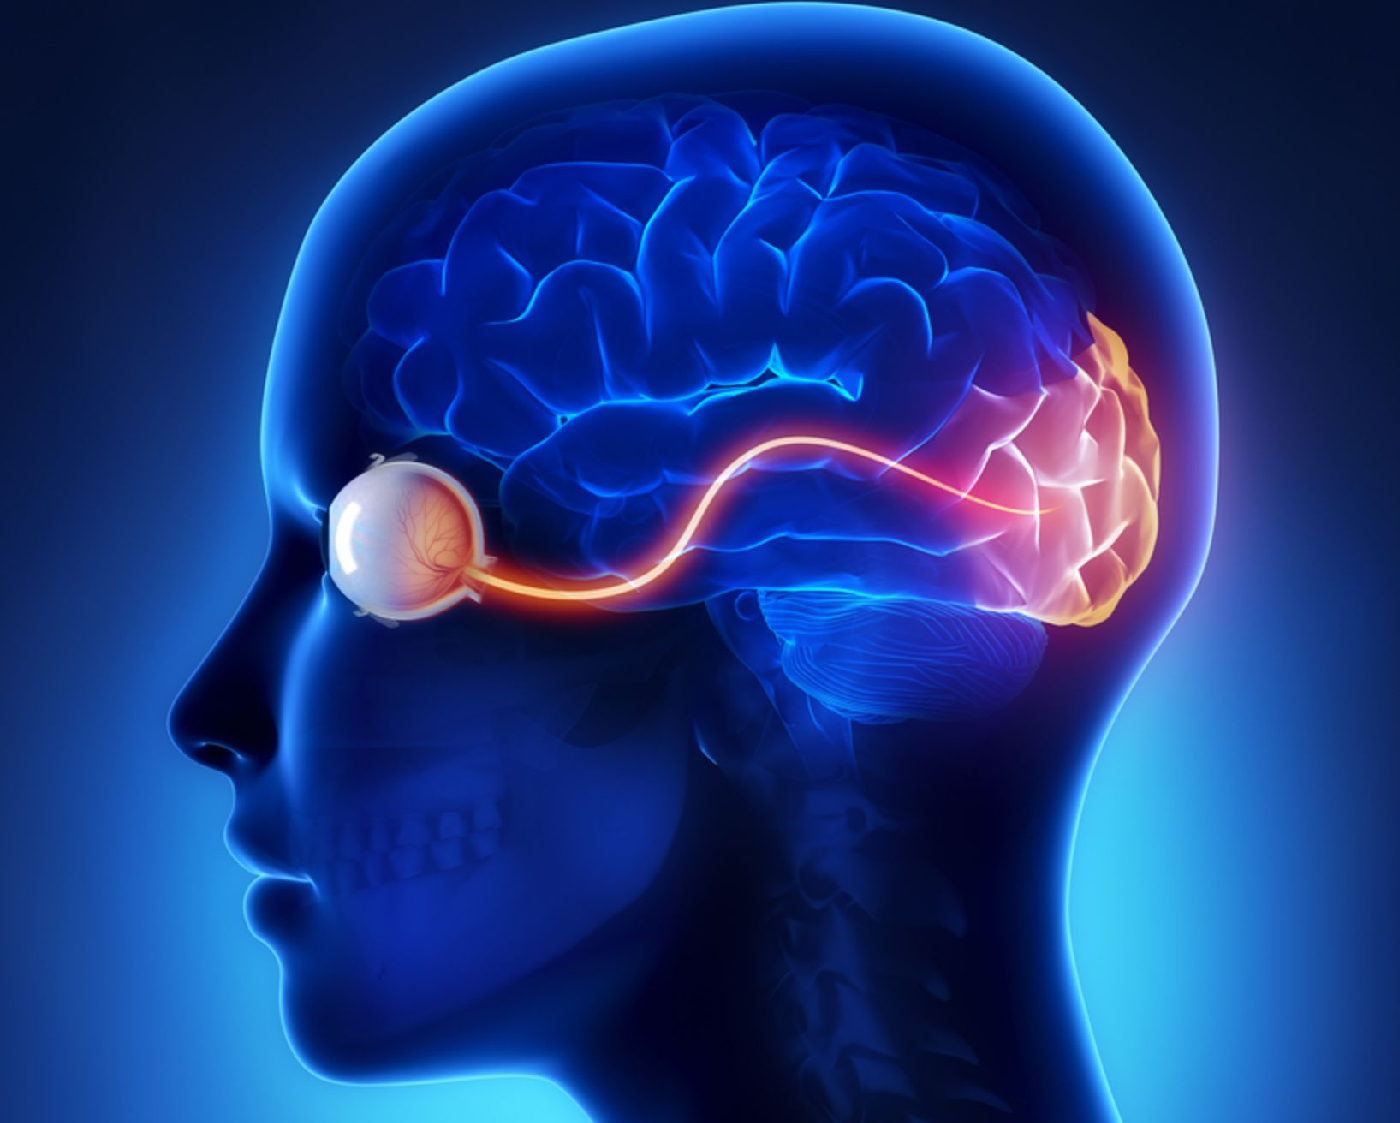
\includegraphics[width=\paperwidth]{images/eye-nerve-brain.pdf}
            };
        \end{tikzpicture}
     \end{frame}
}

%------------------------------------------------

\begin{frame}
\frametitle{Vision}

\Large Vision, of our all senses, is the most powerful and efficient 
{\hilit channel for receiving information} from the physical world.

\end{frame}

%------------------------------------------------

\begin{frame}
\frametitle{Importance of Vision}

\bbi
  \item Vision dominates our senses
  \item Most powerful channel for receiving information
  \item About half of the human brain deals with visual input
  \item $\sim$ 70\% of the sense receptors in our bodies are dedicated to vision
  \item It is the sense most connected with cognition
  \item Seeing and thinking are extremely related: \\
  how we see $\Leftrightarrow$ how we think
\ei

\end{frame}

%------------------------------------------------

\begin{frame}
\frametitle{Vision}

\bb{So many ways to see ...}
``There are so many ways for speakers of English to see the world. We can glimpse, glance, visualize, view, look, spy, or ogle. Stare, gawk, or gape. Peek, watch, or scrutinize. Each word suggests some subtly different quality: looking implies volition; spying suggests furtiveness; gawking carries an element of social judgment and a sense of surprise.''
\eb

\textit{Joshua Foer (Utopian for Beginners)}

\end{frame}

%------------------------------------------------

\begin{frame}
\frametitle{Seeing and Thinking}
\begin{center}
\ig[width=11cm]{images/eye-and-brain.pdf}
\end{center}
\end{frame}

%------------------------------------------------

\begin{frame}
\frametitle{Seeing}

\bb{What our eyes get is not what our brain perceives}
What we commonly call ``seeing'' is not a single phenomenon but a group of
at least 3 operations:
\bi
  \item Sight
  \item Perception
  \item Cognition
\ei
\eb

\end{frame}

%------------------------------------------------

\begin{frame}
\frametitle{How we see}
\begin{center}
\ig[width=11cm]{images/how-we-see.pdf}
\end{center}
\end{frame}

%------------------------------------------------

\begin{frame}
\frametitle{Visual Perception}

\bb{Making sense of what our eyes see}
``We don't see with our eyes; we see with our brains. Our eyes are the sensory
mechanisms through which light enters and is translated by neurons into
electrical impulses that are passed on to and around in our brains, but our
brains are where perception actually occurs.''
\eb

\textit{Stephen Few (Information Dashboard Design)}

\end{frame}

%------------------------------------------------

\begin{frame}
\frametitle{Psycho-Physical System}
\begin{center}
\ig[width=11cm]{images/psychophysical-system.pdf}
\end{center}
\end{frame}

%------------------------------------------------

\begin{frame}
\frametitle{Visual System}

\bbi
  \item The visual system consists of 2 parts
  \bi
    \item eyes
    \item brain
  \ei
  \item The \textbf{eyes} act as image receptors
  \item The \textbf{brain} acts as an image processing and interpreation unit
  \item Understanding how we see requires that we understand both components
\ei

\end{frame}

%------------------------------------------------

\begin{frame}
\frametitle{Electromagnetic Spectrum}
\begin{center}
\ig[width=11cm]{images/visible-spectrum.pdf}
\end{center}
\end{frame}

%------------------------------------------------

\begin{frame}
\frametitle{A little bit about Light}

\bbi
  \item Light is electromagnetic radiation
  \item Light can be described as waves that scatter in different lengths,
  frequencies, and energy charges
  \item Our eyes detect only a tiny fraction of the electromagnetic spectrum
  \item The visible range for humans runs from violet to red
\ei

\end{frame}

%------------------------------------------------

\begin{frame}
\begin{center}
\Huge{\hilit{Anatomy of the Eye}}
\end{center}
\end{frame}

%------------------------------------------------

{ % all template changes are local to this group.
    \begin{frame}[plain]
        \begin{tikzpicture}[remember picture,overlay]
            \node[at=(current page.center)] {
                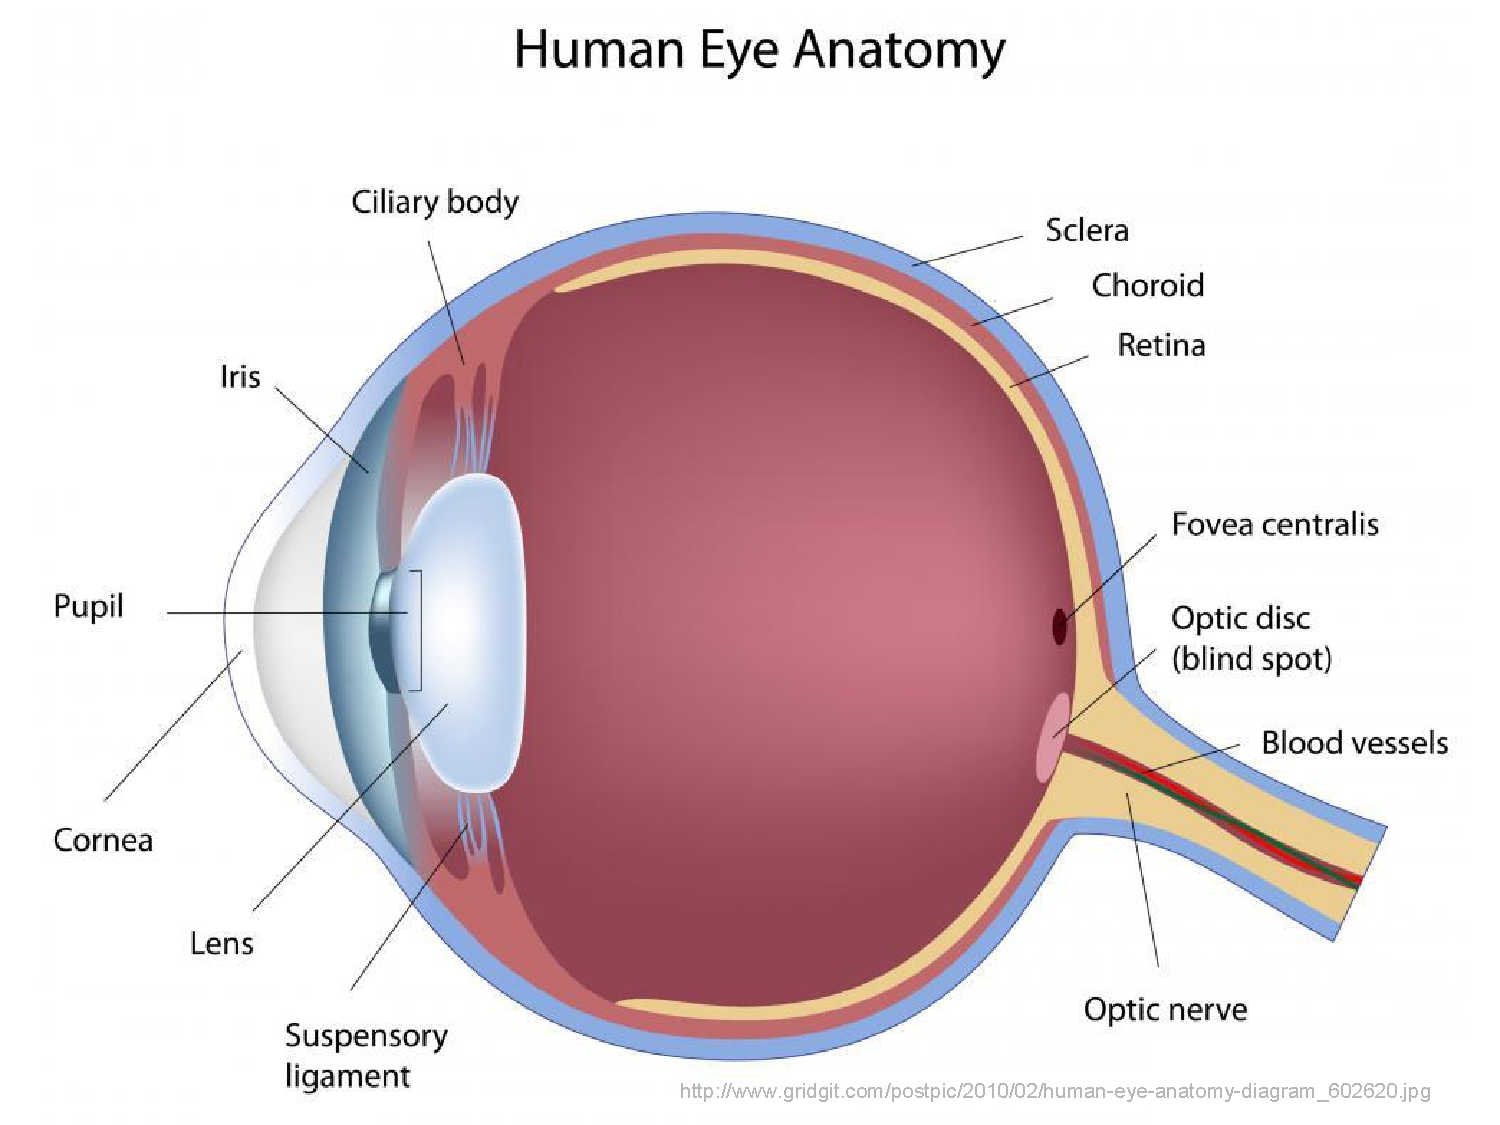
\includegraphics[width=\paperwidth]{images/eye-anatomy.pdf}
            };
        \end{tikzpicture}
     \end{frame}
}

%------------------------------------------------

\begin{frame}
\frametitle{Mechanics of eye and sight}

\bbi
  \item To better understand how we ``see'', we should talk about the eye.
  \item Knowing about the physiology of the eye is fundamental to better
  design visual displays and statistical graphics.
\ei

\end{frame}

%------------------------------------------------

\begin{frame}
\begin{center}
\ig[width=11cm]{images/eye-anatomy-cornea.pdf}
\end{center}
\end{frame}

%------------------------------------------------

\begin{frame}
\frametitle{Outside layers of the eye}

\bb{Cornea}
\bbi
  \item The surface of the eye is called the \textbf{cornea}.
  \item The cornea is a protective covering.
  \item It is the transparent, dome-shaped window covering
  the front of the eye. 
  \item It is a powerful refracting surface, providing 2/3
  of the eye's focusing power.
\ei
\eb

\end{frame}

%------------------------------------------------

\begin{frame}
\frametitle{Outside layers of the eye}

\bb{Sclera and conjuctiva}
\bbi
  \item The \textbf{sclera} is ``the white of the eye.'' It is the tough, 
  opaque tissue that serves as the eye's protective outer coat.
  \item The \textbf{conjunctiva} is the thin, transparent tissue that covers
  the outer surface of the eye.
\ei
\eb

\end{frame}

%------------------------------------------------

\begin{frame}
\begin{center}
\ig[width=11cm]{images/eye-anatomy-iris.pdf}
\end{center}
\end{frame}

%------------------------------------------------

\begin{frame}
\frametitle{Outside layers of the eye}

\bb{Iris and Pupil}
\bbi
  \item Behind the cornea resides the \textbf{iris}.
  \item The iris is a colored muscle that works like a camera shutter.
  \item It covers all but a small opening in the front of the eye.
  \item The \textbf{pupil} is the opening at the center of the iris.
  \item The iris enlarges or decreases the size of the pupil.
\ei
\eb

\end{frame}

%------------------------------------------------

\begin{frame}
\frametitle{Outside layers of the eye}

\bb{Iris and Pupil}
\bbi
  \item The iris controls the amount of light entering the eye.
  \item In low-light conditions the pupil dilates to let in more light.
  \item In high-light conditions the pupil constracts to let in less light.
  \item The size of the pupil is also subject to mood. It dilates when we are
  happier.
\ei
\eb

\end{frame}

%------------------------------------------------

\begin{frame}
\begin{center}
\ig[width=11cm]{images/eye-anatomy-lens.pdf}
\end{center}
\end{frame}

%------------------------------------------------

\begin{frame}
\frametitle{Focus Control}

\bbi
  \item The cornea and aqueous humour act as a primary lens which performs
  crude focusing of the incoming light.
  \item Behind the iris there is the \textbf{lens}, similar to the lens of
  a camera
  \item The \textbf{lens} is made of a soft transparent substance. It provides
  control over the eye's focusing.
  \item With age, the lens gradually hardens making it harder for the eye to
  focus on nearby objects.
\ei

\end{frame}

%------------------------------------------------

\begin{frame}
\begin{center}
\ig[width=11cm]{images/eye-anatomy-back.pdf}
\end{center}
\end{frame}

%------------------------------------------------

\begin{frame}
\frametitle{Retina}

\bbi
  \item The \textbf{retina} is a thin sheet of nerve tissue at the back of the 
  eye.
  \item The retina is not really part of the eye but part of the brain.
  \item It is composed of more than 100 million light-absorbing receptors.
  \item Its job is to convert this light energy into electrical impulses
  for the brain to interpret.
\ei

\end{frame}

%------------------------------------------------

\begin{frame}
\frametitle{Retina Cell Receptors}
\begin{center}
\ig[width=11cm]{images/eye-rods-cones.pdf}
\end{center}
\end{frame}

%------------------------------------------------

\begin{frame}
\frametitle{Retina Cell Receptors}

\bbi
  \item Two kinds of nerve cells live in the retina: rods and cones
  \item The retina has about 100 million rods, and 7 million cones
  \item Rods control our ability to see in low light
  \item Cones control our color and detail vision
  \item Photosensitive chemicals in the rods and cones cause an electrical
  reaction that sends seen images through optic nerves to the brain's cerebral
  cortex
\ei

\end{frame}

%------------------------------------------------

\begin{frame}
\frametitle{Photosensitive Cells}
\begin{center}
\ig[height=7cm]{images/rods-cones-cells.pdf}
\end{center}
\end{frame}

%------------------------------------------------

\begin{frame}
\frametitle{Rod cells}

\bbi
  \item Rods come in only one type.
  \item Most sensitive type of photoreceptor cells.
  \item Provide low-light vision (night vision).
  \item Provide no color discrimination.
  \item Operate within light spectrum between 400 and 700 nm.
\ei

\end{frame}

%------------------------------------------------

\begin{frame}
\frametitle{Cone cells}

\bb{Three types of cell cones}
\bbi
  \item \textbf{S} (short wavelength)
  \item \textbf{M} (medium wavelength)
  \item \textbf{L} (long wavelength)
  \item The cone types combine to help us see the range of visible color.
\ei
\eb

\end{frame}

%------------------------------------------------

\begin{frame}
\frametitle{Cones light sensitivity}

\bb{Spectrum Peaks}
\bbi
  \item Each cone is most sensitive to light in a different wavelength.
  \item \textbf{S} cones peak at 420 nm
  \item \textbf{M} cones peak at 530 nm
  \item \textbf{L} cones peak at 560 nm
\ei
\eb

\end{frame}

%------------------------------------------------

\begin{frame}
\frametitle{Rods and Cones}

\bbi
  \item The distribution of rod and cone cells is not uniform across the retina.
  \item The cones are concentrated at the center rear of the retina.
  \item The rods are more evenly distributed away from the retina.
\ei

\end{frame}

%------------------------------------------------

\begin{frame}
\frametitle{Rods and night vision}

\bbi
  \item In very low light or at night we see using only our rods.
  \item At night we have a blind spot at the center of our visual field.
\ei

\end{frame}

%------------------------------------------------

\begin{frame}
\frametitle{Retina Cell Receptors}
\begin{center}
\ig[width=11cm]{images/rods-and-cones.pdf}
\end{center}
\end{frame}

%------------------------------------------------

\begin{frame}
\frametitle{Orientation of Photosensitive Cells}

\bbi
  \item Once the light passes through the pupil, it shines on the retina.
  \item Layer of cells that makes up the retina is backwards.
  \item Light rays must pass through neurons and optic nerve fibers first.
  \item Then the rays reach the photosensitive cells.
  \item Rods and cones are also facing away from the light source.
  \item In summary: the eyes are actually part of the brain.
\ei

\end{frame}

%------------------------------------------------

\begin{frame}
\frametitle{About human vision}

\bb{Sight Mechanics in a nutshell}
Light delivers images and colors to the brain through nerve cells,
in the retina of the eye. To get to the retina at the back of the eye, images
and colors travel through various layers.
\eb

\end{frame}

%------------------------------------------------


\begin{frame}
\begin{center}
\Huge{\hilit{The Visual Brain}}
\end{center}
\end{frame}

%------------------------------------------------

\begin{frame}
\frametitle{Visual Pathways}
\begin{center}
\ig[width=10cm]{images/visual-pathways.pdf}
\end{center}
\end{frame}

%------------------------------------------------

\begin{frame}
\frametitle{Visual Pathways}

\bbi
  \item After light has entered the eye, it is filtered and adjusted
  \item Then it reaches the retina (at the back of the eye)
  \item The retina contains nerve cells that are sensors designed to absorb
  light and translate it into neural signals
  \item The neural signals are then passed via the optic nerve to our brains
  \item They are processed in the region of the brain called the visual cortex
\ei

\end{frame}

%------------------------------------------------

\begin{frame}
\frametitle{Transmission to the Cortex}

\bbi
  \item The visual signal from the retina is transmitted down the optic nerve.
  \item There are roughly 1 million nerve fibers in the optic nerve, and around
  125 million photoreceptors in the retina.
  \item The signal is not transmitted in a one-fiber per receptor fashion.
  \item The greatest convergence occurs for the rod cells: the signals from 
  1000 rods may be carried by the same nerve fiber.
  \item This implies that there some ``data compression'' processing.
\ei

\end{frame}

%------------------------------------------------

\begin{frame}
\frametitle{The Optic Chiasm}

\bbi
  \item The optic nerves from the two eyes converge and cross at the structure
  called the \textbf{optic chiasm}.
  \item Signals form each eye are mixed at this point.
  \item Such combination is necessary for filling-in the blind spot and for
  comparison leading to the extraction of depth information.
\ei

\end{frame}

%------------------------------------------------

\begin{frame}
\frametitle{Visual Brain}

\bbi
  \item The retina receives electrical patterns and creates several tracks 
  from the patterns
  \item Some tracks contain information about shadows, others about movement,
  and so on
  \item As many as 12 tracks of information are then sent to the brain's
  visual cortex
  \item Different regions of the visual cortex respond to and process the
  information of the tracks.
\ei

\end{frame}

%------------------------------------------------

\begin{frame}
\frametitle{The Visual Cortex}

\bbi
  \item The visual cortex contains a number of neural structures which extract
  basic information from the visual signal.
  \item There are groups of neurons which are dedicated to detecting lines
  with particular orientation.
  \item Other groups are dedicated to detect shapes.
  \item The signal is processed at higher and higher levels and eventually
  passed forward to the higher brain centers.
\ei

\end{frame}

%------------------------------------------------

\begin{frame}
\frametitle{Retina is part of the brain}

\bbi
  \item There is about 120 million rods and 6 million cones.
  \item The optic nerve only contains about 1 million fibers.
  \item Not all the visual information is transmitted to the brain.
  \item The eye performs a significant amount of visual processing.
  \item Compressed information is sent via the optic nerve.
\ei

\end{frame}

%------------------------------------------------

\begin{frame}
\frametitle{Visual Brain}

\bbi
  \item What your eyes physically perceive is only one part of the equation
  \item What you see isn't what your brain gets
  \item The images coming to your brain are processed and interpreted
  \item It is really your brain that is ``seeing''
\ei

\end{frame}

%------------------------------------------------

\begin{frame}
\begin{center}
\Huge{\hilit{Foveal and Peripheral Vision}}
\end{center}
\end{frame}

%------------------------------------------------

\begin{frame}
\frametitle{The Blind Spot}

\bbi
  \item There are no photoreceptors where the optic nerve reaches the retina.
  \item This creates a blind spot in the visual field of each eye.
  
  \item We are usually unaware of our blind spots because information from the 
  other eye is used to fill in the missing part of the visual field.
\ei

\end{frame}

%------------------------------------------------

\begin{frame}
\frametitle{Finding your blind spot}

\bi
  \item Draw a cross and a dot about 8 cm apart as shown below.
  \item Close your right eye.
  \item Look directly at the cross.
  \item Move the page backward and forward until you see the dot disappear.
\ei

\begin{center}
\ig[width=9cm]{images/blind-spot.pdf}
\end{center}

\end{frame}

%------------------------------------------------

\begin{frame}
\frametitle{Foveal and Peripheral Vision}

\bbi
  \item Most visual information falls in the peripheral areas of the retina
  \item There is one special region in the retina called the fovea 
  \item It is the place that provides the sharpest vision
  \item The fovea allows us to distinguish small objects, detail, and color
  \item Our eyes repeatedly move to keep the object of most interested imaged
  on the fovea
\ei

\end{frame}

%------------------------------------------------

\begin{frame}
\frametitle{Vision Fields}
\begin{center}
\ig[width=11cm]{images/vision-fields.pdf}
\end{center}
\end{frame}

%------------------------------------------------

\begin{frame}
\frametitle{Foveal and Peripheral Vision}

\bbi
  \item Most visual information falls in the peripheral areas of the retina.
  \item There is one special region in the retina called the fovea.
  \item It is the place that provides the sharpest vision.
  \item The fovea allows us to distinguish small objects, detail, and color.
  \item Our eyes repeatedly move to keep the object of most interested imaged
  on the fovea.
  \item The central vision is critical for specific object recognition.
  \item Peripheral vision is used for getting the gist of a scene.
\ei

\end{frame}

%------------------------------------------------

\begin{frame}
\frametitle{What your brain thinks you are seeing}
\begin{center}
\ig[width=10cm]{images/focus-normal.pdf}
\end{center}
\end{frame}

%------------------------------------------------

\begin{frame}
\frametitle{What your eyes are really getting}
\begin{center}
\ig[width=10cm]{images/focus-flowers.pdf}
\end{center}
\end{frame}

%------------------------------------------------

\begin{frame}
\frametitle{What your eyes are really getting}
\begin{center}
\ig[width=10cm]{images/focus-bench.pdf}
\end{center}
\end{frame}

%------------------------------------------------

\begin{frame}
\frametitle{What your eyes are really getting}
\begin{center}
\ig[width=10cm]{images/focus-path.pdf}
\end{center}
\end{frame}

%------------------------------------------------

\begin{frame}
\begin{center}
\Huge{\hilit{Foveal and Peripheral Vision}}
\end{center}
\end{frame}

%------------------------------------------------

\begin{frame}
\frametitle{Herman Grid Illusion}
\begin{center}
\ig[width=10cm]{images/herman-grid.pdf}
\end{center}
\end{frame}

%------------------------------------------------

\begin{frame}
\frametitle{Unexpected Visitors by Ilya Repin (1884-1888)}
\begin{center}
\ig[width=10cm]{images/unexpected-visitors.pdf}

{\lolit \scriptsize{https://www.wikiart.org/en/ilya-repin/unexpected-visitors-1888}}
\end{center}
\end{frame}

%------------------------------------------------

\begin{frame}
\frametitle{Eye tracking experiments by Alfred Yarbus}
\begin{center}
\ig[height=7cm]{images/unexpected-visitors-tracking.pdf}

{\lolit \scriptsize{Wikimedia commons: Yarbus The Visitor}}
\end{center}
\end{frame}

%------------------------------------------------

\begin{frame}
\begin{center}
\Huge{\hilit{Takeaways}}
\end{center}
\end{frame}

%------------------------------------------------

\begin{frame}
\frametitle{Main takeaways}

\bbi
  \item We use both peripheral and central vision when looking at an image.
  \item Don't assume people will see something on a graphic just because it's
  there.
  \item Avoid putting important things on the edges, since we tend not to
  look there.
  \item About short-term memory: viewers of graphs can only hold a few chunks
  of information in their heads at any one time.
\ei

\end{frame}

%------------------------------------------------

\begin{frame}
\frametitle{References}

\bbi
  \item \textbf{The Functional Art} (chapter 5) by Alberto Cairo.
  \item \textbf{Visual Language for Designers} (section 1) by Connie Malamed.
  \item \textbf{Now You See It} (chapter 3) by Stephen Few.
  \item \textbf{Show Me the Numbers} (chapter 6) by Stephen Few.
  \item \textbf{Interactive Data Visualization} (chapter 3) by Ward, Grinstein
  and Keim.
  \item \textbf{100 Things Every Designer Needs to Know About People} 
  (chapter 1) by Susan M. Weinschenk.
\ei

\end{frame}

%------------------------------------------------

\end{document}
